\chapter{Methods}
\label{sec:methods}

The general issue of utilizing grid computing or cloud computing infrastructure is to select appropriate method to integrate domain specific computation into the grid or cloud infrastructure of a concrete provider. 

A lot of tools are already available within current grid infrastructure including open-source or licensed software for computation. A list of available application is usually given by the local scientific provider\footnote{applications available in CESNET METACENTRUM \url{https://wiki.metacentrum.cz/wiki/Kategorie:Applications} accessed February 2015} or application database are available in broader environment e.g. in EGI.eu application database\footnote{\url{https://appdb.egi.eu/} accessed February 2015}.
Additionaly workflow systems and scientific gateways mentioned in section \ref{sec:introworkflow} tries to hide the complexity of grid-computing or cloud-computing infrastructure and may be used to integrate specific domain too.
The programming model of parallel computing and/or distributed  computing (in section \ref{sec:parallelprogramming} and  \ref{sec:distributedprogramming}) needs to be followed when designing new application utilizing benefits of grid-computing and/or cloud computing.

The general approach to port application to grid infrastructure is to automatize what can be automatized, i.e. make scripts, configure system, prepare some UI, integrate with existing applications, utilize protocol compatibility etc. An effort to obtain first results is high, however for further computational request, the prepared templates, scripts are reused and effort is much lower.  

\section{Sharing medical information}
\label{sec:imaging}
%\label{sec:medicalapp}
%Acquiring, storing and processing digital medical images 
%This chapter introduces acquiring, storing and sharing digital medical images and related metadata within hospital or healthcare provider and among them and research institution.

%are covered in section \ref{sec:introimages}. Overview of analysis of speech and voice and it's relation to voice science is in section \ref{sec:introvoice}. Overview of models and simulation of human physiology and it's relation to systems biology is briefly covered in section \ref{sec:intromodels}.


%The computing in biomedicine can be divided into research and clinical application. %Translational science aims to "translate" findings from research to better health care including diagnostic tools, procedures, drugs, etc.

%In case of research use-cases, processing medical information helps to make more precise current theories or support formulating new one. In case of clinical use cases, processing medical information helps to analyse and interpret the information, predicting future trends and support decision on some intervention.

%\footnote{Motivation of using distributed computing technologies is to share physical data, among multiple organizations, where there is no need or other barriers to store all data centrally, e.g. for legal or capacity limitation. A lot of medical information within biomedical research came from real patient and such information are protected by some regulation and processing of them is regulated and controlled by the country laws or international agreements. Thus there must be considered ethical as well as legal issues how to deal with such information. Sharing and processing of medical images are covered in section \ref{sec:introimages}. Providing access to services with high values is another motivation of using distributed computing technologies. E.g. basic and advanced analysis of biological signals, especially of voice is described in section \ref{sec:introvoice}.}


Use cases related to digital medical images involves the image acquisition, preprocessing, storing and searching.
Clinicians use patient image mainly for visualization and diagnostic purposes. Computer assisted methods facilitate the diagnostic process and involves image enhancement (to reduce image noise and increases the contrast), image segmentation (to separate different types of structures from background and from each other), quantification methods (to determines the structure shape, size, volume), registration methods (to process and join multiple different images into one).
Comprehensive concepts and digital techniques in medical imaging are presented e.g. in book edited by I.N.Bankman\cite{Bankman2000}.

Acquisition of the medical image is covered with different modalities (different types of equipment and sensors) by radiologists or other specialists. DICOM\footnote{DICOM: \url{http://dicom.nema.org/} accessed January 2015} format and protocol becomes the de-facto an industrial standard to exchange medical images electronically and picture archiving communication systems (PACS) holding the acquired DICOM images with metadata and description noted by experts are currently part of information systems in hospitals. See the typical workflow of medical image in hospital in fig. \ref{fig:pacs}.

\begin{figure}[ht]
    \centering
    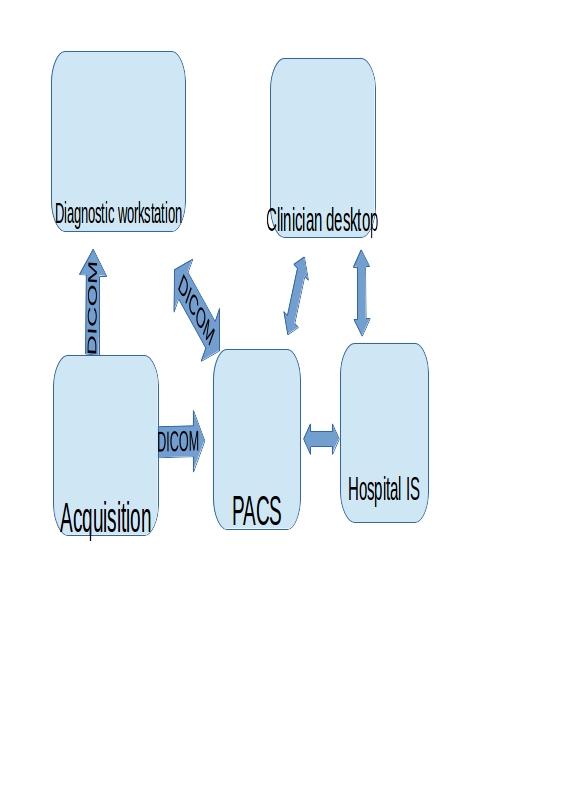
\includegraphics[width=0.8\textwidth, height=8cm]{chapter4/pacs.png}
    \caption{Typical workflow of medical image in hospital. Data acquisition is made by modalities (magnetic resonance, ultrasonography, X-ray radiography, etc.) and using DICOM format and protocol it can be directly transferred and visualized by diagnostic workstation. With metadata filled by an expert physician the image is stored in PACS. Other desktops within hospital can retrieve the image and review the report. The hospital information system may be involved in other workflows and communicate with other formats and standards (HL7,...)
    }
    \label{fig:pacs}
\end{figure}

As the data processed in hospital information systems contains sensitive information of real patients, these are protected and processing and storing is regulated by the national or international laws or agreements.
Development of telecomunication and network technologies a enabled telemedicine -- providing healthcare over remote distance. It requires to share and exchange  sensitive data of real patient among different helthcare providers and additionaly such data may be very valuable for further research. Security and encryption should be addressed and DICOM standard itself doesn't solve security issues appropriately, thus encyption during transferring the data over computer network must be ensured by other techniques.

In the Czech Republic, there exists several projects in production interconnecting different hospitals, clinics and other healthcare organization to exchange medical images. Project ePACS allows interconnecting each participant's PACS system via dedicated VPN channel to the central node and exchange of medical images are realized by routing the data flow from one VPN channel to the other\footnote{ePACS:\url{http://www.epacs.cz}, accessed January 2015}. Another approach is used in the project MEDIMED held by Masaryk University in Brno. Instead of dedicated VPN channel, they use  SSL encryption over standard TCP/IP communication and regional hospitals and healthcare providers are interconnected via the MEDIMED servers \cite{Slavicek2010}.% \cite{Javornik2011,Zatloukal2012}.
In other countries, there were tested cross-border teleradiology in projects Baltic e-health, R-Bay and others \cite{Ross2010,Saliba2012}.
These projects are focused on sharing the medical images and other knowledge and information.

Access to the wide range of medical images is needed for research of new processing and diagnostic methods, rare diseases, developing new detection algorithm etc.  DICOM records "de-identified" (identification of patient records are deleted, only date of the bird and other data are kept) or anonymized (additional information are manipulated to prevent disclosure) for research purposes to protect sensitive personal data, but keep important information for research purposes. The Globus MEDICUS project published by Erberich et al.\cite{Erberich2006,Erberich2007} is based on Globus Toolkit middleware to federate clinical and research application via a grid-computing infrastructure. Currently the project is hibernated since 2008 and no further development was published\footnote{\url{https://dev.globus.org/wiki/Incubator/MEDICUS} accessed February 2015}. Similar effort was done with a project Medical Data Manager which uses gLite grid middleware published by Duque, Montagnat et al.\cite{Duque,Montagnat2007} \footnote{\url{http://modalis.i3s.unice.fr/softwares/mdm/start} accessed February 2015} or MediGRID project published by Krefting et al.\cite{Krefting2009, Krefting2010}. Additionally to the sharing medical images, processing of images within selected use-cases supported by the grid-computing infrastructure is introduced\cite{Krefting2010}. Health-e-child project aimed to interconnect research institution and hospitals in UK, France and Italy for the purpose of grid-based healthcare platform for pediatric health-care \cite{Skaburskas2008}. Neurist project developed architecture and connects clinicians and researchers to improve research and treating of cerebral aneurysm to provide tools to analyze and interpret patient data and researcher can have access to set of aneurysm data, published by Benkner et al.\cite{Benkner2010}.
SEAGRIN research project aimed to  share knowledge mainly for educational purposes in semi-formally described semantics and such proposal and implementation was published by Kuba et al.\cite{Kuba2006}. 

Storing the sensitive medical information even de-identified or anonymised is usually restricted and this lead to an idea to store such information within trusted institution e.g. hospital and move and facilitate deployment of the grid services storing medical data to that institution. E.g. pre-installed virtual machines can contain grid-services and deployed in as a sealed grid as proposed by Kuba et al. \cite{Kuba2007a}.


%When we look to the architecture of the systems of sharing medical images the problematic part within the point-to-multipoint architecture is the central part of the systems already in production e.g. in Czech Republic (MEDIMED, ePACS). This may become single point of failure and bottleneck.

To summarize this section, digital medical image acquisition, store, exchange and processing became common in the past years and is currently using distributed computing techniques. There are several efforts to implement medical data management within grid or cloud infrastructure for research purposes and integrate them with the production infrastructures. Security is solved by authentication, authorization mechanism as well as by encrypting the data and/or de-identification or anonymization but keeping minimal information required for research purpose. A related question is  how easily the previously mentioned grid-based technologies can be integrated with current systems in hospitals or institutions. The following section describes selected methods used to integrate a pilot deployment of Globus MEDICUS with current regional system for exchanging medical images - MEDIMED.

\subsection{Methods to share medical images in grid}
\label{sec:methodsimages}

Globus toolkit belongs to the group of most used grid middleware (see section~\ref{sec:servicegrid}). The core services included in Globus Toolkit are GridFTP -- grid extension to file transfer protocol(FTP) implements strategies such as \emph{stripping data} into multiple pieces, \emph{parallel transfer of data} utilizing stripped data parts to be transfered via different channels, \emph{partial file transfer} some application may not need to acess the whole file, but a smaller portion of it. etc. \cite{Foster2006, Allcock2005}. Other core services are Replica Location Service aiming to localize data, Globus Resource Allocation Management (GRAM) provides web service and proxies to the lower level job schedulers implementation \cite{Foster2006}.

Next to core services, the domain specific services might be implemented for the purpose of application using the open grid service architecture (OGSA). Globus MEDICUS \cite{Erberich2006,Erberich2007} contains a DICOM Grid Interface Service (DGIS) and integrates the open source PixelMed\texttrademark ~Java DICOM Toolkit\footnote{\url{http://www.pixelmed.com/} accessed February 2015} into a web service communicating via DICOM protocol and on the other side it forwards the queries to underlying services within Globus toolkit. 

DGIS behaves as a gateway to a grid infrastructure. Because communication via DICOM protocol is not secured, the DGIS is recommended to be installed on the location of the PACS system or DICOM ready modality or software.
When a DICOM study is uploaded into DGIS, it is anonymized and stored and a record is made into another services Meta Catalog service which resides in the same domain or anywhere in grid accessible via Globus Toolkit.
Such anonymized database of DICOM records can be used to query via DGIS interface and to e.g. integrate with web based application showing records for research purposes, authentication and authorization can be done in this level. 
To integrate this system with existing system for sharing the medical images (e.g. the MediMed project\cite{Slavicek2010}) the special client software "RediMed console" needs to be installed next to the DGIS and configured it as a local PACS system whose records might be exchanged to other MediMed participants. 
The results of this particular deployment and integration is in section \ref{sec:resultsimages}.
%The software for processing medical images can retrieve them from DGIS via DICOM protocol. 

%To present DICOM studies The integration strategy based on shared database or files can be used to present the DICOM studies via web portal. Additionally the web portal might generate specific DICOM queries to DGIS.


%The following section will cover methods related to the integration effort.

%The section~\ref{sec:introintegration} describes several general software architectural styles and integration patterns used in further in this work. 
%The section~\ref{sec:methodsimages} describes specific methods used in the area of processing  medical images within grid infrastructure to verify the integration effort between research and hospitals systems. The section~\ref{sec:methodsvoice} describes a method to deploy existing application as a service to the distributed infrastructure.The section~\ref{sec:methodsmodels} focus on modelling methodology in order to build and maintain complex models of human physiology as the complex models seems to mainly benefit from parallel computation. And the subsection~\ref{sec:methodsmodelsestimate} follows up on the modeling methodology to describe the system for estimating model parameters. 

%as a program to start within remote session and , the interactive application allows select type of voice which will be analysed. After recording is finished, the whole recording is analyzed with FFT to obtain full spectral analysis. 

%\section{Integrating heterogenous systems}
%\label{sec:introintegration}
%
%Integrating heterogenous system into a well designed enterprise application has some issues which needs to be addressed.
%
%One of the first decision which may be hard to change in future is platform. Platform might be determined by third party platform-specific product incorporated in a workflow which cannot be changed. There exists software platforms that may run on different operating systems. E.g. Java platform is based on the idea that a program is compiled into bytecode which is then interpretted by just-in time compilers on target platform. Similar approach applies to Common Language Infrastructure (CLI) known by it's implementation .NET Framework on Microsoft Windows operating system or MONO which is implemented on Linux platforms.
%Another approach to address the issue of a platform is virtualization as mentioned already in section \ref{sec:introvirtual}.
%
%
%%\subsection{File exchange}
%Is based on the fact, that one process produces a file which is consumed by another process. This is popular in batch processing systems which needs no or only limited interactivity with user. The grid workflow management systems 
%\subsection{Message Oriented Integration}
%The processes that run concurently synchronize and exchange messages via some dedicated channel. E.g. platform depended
%
%\subsection{Service Oriented Architecture}
%\label{sec:methodssoa}
%Service oriented architecture (SOA) decouples a service contract with intention to be platform independent from it's platform-dependent implementation\cite{Erl2008}. The loosely coupled modules conforming the SOA style are realized as web service which contracts are described in Web Service Definition Language (WSDL) which defines the service interface in term of endpoint location (URL), sset of operation, binding of operation to endpoint, the format of input and output messages and binding of the messages to the operations. These are usually based on some XML dialect. Even the WSDL can be written by hand, it can be generated by a service stack framework for the concrete service implementation. 
%Next to the service implementation there are abstraction like registry and repository holding metadata of the service, so it can be dynamically discovered.
%
%\subsection{RESTful web services}
%\label{sec:methodsrest}
%The Representational State Transfer (REST) architectural style proposed by R. Fielding\cite{fielding2000chapter} is used for representing functionality as a limited  for solving demand issues of the selected tasks 
%

%The images produced by medical devices are mainly in a DICOM standard which describes the file format and communication protocol for exchange, query/retrieve image, modality and other metadata \cite{dicom2011}. The file format consist of header which involves information about the patient and the pixel data containing uncompressed or compressed bitmap of image. Some devices produces multi-frame multi-dimensional images which can be stored in one DICOM file. The DICOM standard is used to interconnect multiple medical devices, local computers and database system which is usually termed as Picture Archiving and Communitation System (PACS). 


%The particular methods used within specific biomedical domains are covered in further chapter section \ref{sec:methodsimages}, \ref{sec:methodsvoice}, \ref{sec:methodsmodels}. 

%This chapter covers general methods which might be utilized in any domain. The section~\ref{sec:introintegration} describes several general software architectural styles and integration patterns and section~\ref{sec:introvirtual} covers virtualization technology.


%The section~\ref{sec:introintegration} describes several general software architectural styles and integration patterns used in further in this work. 
%The section~\ref{sec:methodsimages} describes specific methods used in the area of processing  medical images within grid infrastructure to verify the integration effort between research and hospitals systems. The section~\ref{sec:methodsvoice} describes a method to deploy existing application as a service to the distributed infrastructure.The section~\ref{sec:methodsmodels} focus on modelling methodology in order to build and maintain complex models of human physiology as the complex models seems to mainly benefit from parallel computation. And the subsection~\ref{sec:methodsmodelsestimate} follows up on the modeling methodology to describe the system for estimating model parameters. 


%\begin{itemize}
%\item{ 
%The \emph{Service Oriented Architecture} (SOA) is high level programming model based on self contained units of functionality and metadata, so the service can be dynamically discovered and used. An important aspect is separated service implementation from it's contract or interface \cite{Erl2008} and is usually realized by web services. %More about SOA is in section \ref{sec:methodssoa}.
%}
%\item{
%The \emph{Representation State Transfer} (REST) specifies several architectural constraints that helps scalability, performance and presents functionality via fixed number of operation and uniform resource location \cite{fielding2000chapter}. %More about RESTful web services is in section \ref{sec:methodsrest}
%}
%\end{itemize}
%
%Software architecture of the distributed systems are studied and some repeating patterns are cataloged e.g. by Fowler et. al\cite{Fowler2003}. Integration patterns are discussed with focus on the ways of connecting heterogenous parts of the system as presents Hohpe et al.\cite{Hohpe2002}.

\section{Voice Science}
\label{sec:voice}
With introduction of objective data analysis and laryngoscopy methods the voice science emphasized the cooperation among  laryngologist, speech pathologist and voice teacher.
The human voice ranges from 50 Hz to something about 1000 Hz, but there are large  individual variation. For analysis of digitally recorded voice, either habitual or singing, the Discrete Fourier Transformation(DFT) is used to produce frequency and amplitude analysis of recorded input voice samples. One of the most used class algorithm to compute DFT is class of Fast Fourier Transformation with computational complexity $O(n \log(n))$ \cite{Cooley1965,Frigo2005}.
% and parallel version of the algorithms may introduce additional speedup for larger samples of analyzed data \cite{Gupta1993,Takahashi2003}. 
The result of analysis can be visualized in a voice range profile and there can be seen significant difference between untrained and trained voice as well as quantitatively seen some disorders  \cite{DeLeoLeBorgne2002,wuyts2003effects}.

Other methods to analyse vocal chords is laryngoscopy. The videostroboscopy and high speed video in laryngoscope methods produce video for analysing the real movement of vocal chords. The videokymography method introduced by Švec et al. complements the videostroboscopy and allows to visualize and analyze movement of vocal cords recorded by high speed camera on standard TV or monitor with an artificial image built from recorded sequence of selected section \cite{Svec1996,Svec2007}. 

In case of recorded sound and further analysis there is a question about how such a service can be integrated in grid-computing or cloud-computing environment to provide access to a complex application for non-technical voice specialists. Additionally, the analytical software was already developed and calibrated for selected sorts of microphones in MS Windows platform \cite{Fric2007,Fric2012}. Therefore I proposed and implemented a method that provides access to the analytical software remotely. The section \ref{sec:methodsvoice} describes how the analytical software was customized with a remote desktop protocol (RDP). Results are described in section \ref{sec:resultsvoice}. Similar approach might be used for processing the video recordings from laryngoscope, however, the practical limits are discussed in section \ref{sec:conclusion}. 

\subsection{Methods for remote analysis of human voice}
\label{sec:methodsvoice}
%One method to provide access to specialized service is via remote access protocols. Secure Shell (SSH) is used to establish secure channel via unsecured network (e.g. the Internet) from SSH client to SSH server providing e.g. remote command-line, remote command execution etc. It is one of the basic method to access the grid infrastructure and submit computational jobs. 
%Another method is to have a web portal and this web portal based on user's input executes command-line batch scripts over SSH, or it can utilize web services to submit computational job.
Terminal access to some remote computational capabilities, e.g. remote command-line or remote execution is another integration strategy to some remote infrastructure. Secure Shell (SSH) is used to establish secure channel via unsecured network (e.g. the Internet) from SSH client to SSH server and it is basic method to access grid-computing infrastructure. 

Remote Desktop Protocol(RDP) is a proprietary protocol for desktop sharing developed primarly in Microsoft Windows platform, however, today clients and servers exists for several other platforms. Next to remote command-line, remote execution it allows to access remote graphical desktop environment. %VNC is sharing protocol to access remote graphical desktop environment\cite{Richardson1998}. 
The software for parameterized Voice Range Profile (ParVRP) and Voice Range Profile in Real time (RealVoiceLab) was already developed and calibrated for selected sorts of microphones in MS Windows platform by Fric et al.\cite{Fric2007,Fric2012}. The implementation is done in MATLAB environment utilizing Signal Processing Toolbox\footnote{\url{http://www.mathworks.com/products/signal/} accessed February 2015}and compiled with MATLAB Compiler and distributed as an executable.

Instead of migrating the application into some compatible platform for grid-middleware, a virtual machine was introduced and access to the software is provided via RDP protocol. RDP itself contains redirection of several services, e.g. sound recording or drive access. Because the default sound recording redirection introduces some sound degradation without control, I proposed, implemented and integrated the custom RDP plugin with the ParVRP and RealVoiceLab software to redirect the sound recording without loss of information. Technical details are in Appendix~\ref{app:remote}. 

The computation of frequencies and amplitude from the recorded samples utilizes Fast Fourier Transformation which has time complexity $O(n\log(n))$ and current implementation are fast on any even modile devices. The benefit from deploying such application in distributed infrastructure is immediate access to updated software and a collection of anonymized records of voice samples with analyzed results for further research and education purposes.

This type of application can be packaged as virtual machine template and configured within different types of cloud infrastructures and together with a script or web portal the on-demand deployment can be automated. The client part (RDP client) needs to connect to the appropriate instance. The results of such deployment are discussed in section~\ref{sec:resultsvoice}.

\section{Computational physiology}
\label{sec:models}
A mathematical formalization of the fundamental knowledge and relation among biological system - mathematical model - is used as a base abstraction to utilize current discoveries of the genomics and proteomics and formalize the knowledge and construct a "Physiome Model". Model by it's definition is simplification of the complex reality.

Constructing the models and integrating them into complex entity which can be used for further purposes is schematically illustrated in fig. \ref{fig:modeling}. The measurements are done in laboratories or in hospitals. Lumped parameter models are usually represented as ordinary differential equations and differential algebraic equations and characterize the reality as topology of discrete elements. The imaging methods for processing and analysis (section \ref{sec:imaging}) are used to construct 3D models from segmentation and generating of mesh representation connected to physical principles. 
\begin{figure}[ht]
    \centering
    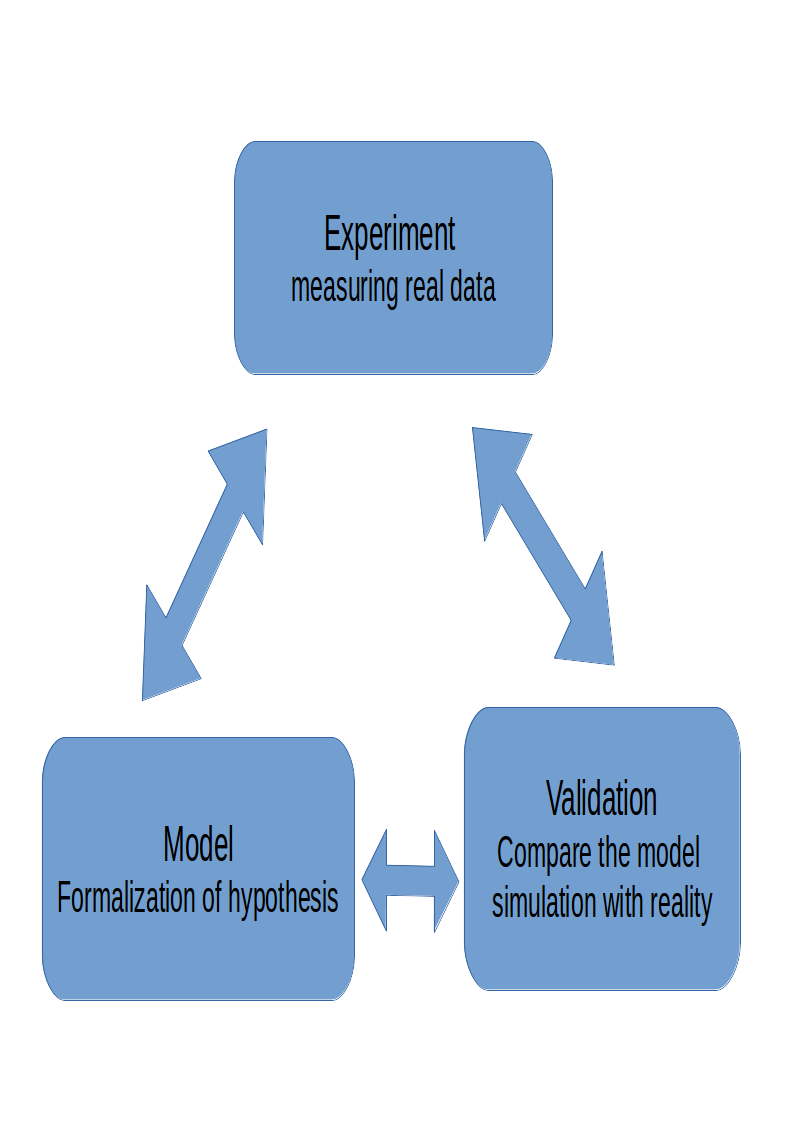
\includegraphics[width=0.5\textwidth, height=5cm]{chapter6/modeling.png}
    \caption{Schematic illustration of scientific process. The experiments produces data which are interpreted and hypothese is formalized as a model. Validation compares the model simulation with experiment, if model satisfies the criteria - is in agreement with real experiments, then the validated model can be used for other purposes.  %\bibentry{EGICompendium2013} \bibentry{egi2014}.
    }
    \label{fig:modeling}
\end{figure}

Application of the mathematical modelling techniques towards the biomedical research is sometimes called as systems biology approach combining the reductionism and integration as denoted by Kohl et al.\cite{Kohl2010}. Application towards the clinical praxis include the quantification of the diagnostic index or treatment strategy and it is a goal to develop tools, database models and methods of several Physiome projects, e.g. VPH-Physiome project presented by Hunter et al.\cite{Hunter2009}.

One of the earliest complex and integrative modelling effort was a model of circulation and it's regulation published by Guyton et al. in 1972 \cite{Guyton1972} which via derivative and technological upgrade continues as "Human Model" or "HumMod" introduced by Hester et al. \cite{Hester2011systems,hester2011} with a focus on integration effort. Different approach of modelling human physiology is a database of smaller models focusing on some particular physiological phenomenon. E.g. the NSR Physiome project introduces  JSIM\footnote{JSIM: \url{http://www.physiome.org/jsim/} accessed January 2015} Java based simulation system to support modeling in  physiology. Repository of several hundred of models were published using this system \cite{Butterworth2014}. The similar effort is done by IUPS Physiome project and repository of models are  based on XML standard languages CellML and FieldML \cite{Hunter2004,Yu2011}. The Systems Biology Markup Language (SBML) is used for modeling biological system at the level of biochemical reaction and regulatory network and another database collects several hundreds of curated and non-curated models \cite{Hucka2004,LeNovere2006}.

JSIM, CellML, SBML or HumMod are domain specific languages and the tools able to work with them are primarily developed within physiological or systems biological communities. Other authors use commercial or industry standard tools for mathematical modelling and computing. E.g. Kofranek et al. describes Guyton's 1972 model in MATLAB\textsuperscript{\textregistered} Simulink \cite{Kofranek2010} and the derivative HumMod in acausal object-oriented Modelica language \cite{Kofranek2011hummod,kofranek2013hummod}. Fernandez et al. describes models of cardiovascular pulsatile system using MATLAB Simscape  \cite{FernandezDeCanete2013} and recently in Modelica  \cite{FernandezdeCanete2014}.

Thus there is an open debate whether in-house domain specific language and tools like JSIM, CellML and FieldML,SBML or HumMod reached it's capabilities for representing complex models. Only the HumMod reached the integrative approach building the complex integrative model of human physiology using lumped parameter approach. I contributed to the idea of key features which involves acausal modeling technique and object orientation which keeps the complex model structure decomposed into understandable and maintainable parts and allows to cover complexity of models like HumMod. 

The methods and examples of modeling cardiovascular system are described in the next section \ref{sec:methodsmodels}. The methods of estimating parameters of complex models are described in section \ref{sec:methodsestimation} and particular results are described in section \ref{sec:resultsestimation}.

%\label{sec:results}
\subsection{Modeling methodology}
\label{sec:methodsmodels}
%For building complex models it seems that acausal (or declarative) modeling technique is key feature as it allows to express the variables declaratively, acausal modeling tool (e.g. Modelica or MATLAB\textsuperscript{\textregistered}  SIMSCAPE\texttrademark) figures out which are the dependent and independent variables upon compilation\cite{fritzson2002}. This allows building complex systems of equation from composed components and the model diagrams still captures the essence of the modeled reality much better and the simulation models are much more legible and thus also less prone to mistakes\cite{Kofranek2008,FernandezDeCanete2013}. 

The methodology of formalizing mathematical models is influenced by the abilities of underlying modeling language used. 
The Modelica language is an object-oriented, equation based and acausal modeling language standardized by Modelica association\footnote{\url{http://www.modelica.org} accessed February 2015}.

%\emph{Object orientation} means that the definition of model is class as in object oriented programming, instance of the model is object,  each instance can share type and differ in parameters and the place where it is used, inheritance and some sort of polymorphism is possible.
%\emph{Equation based} means that the equation is not statement, thus the relation among variables can be expressed in any form and Modelica tool will decide which one is input and output upon compilation. %E.g. from the equation $q = \frac{dV}{dt}$ the process of computation can lead to $ q:= der(V)$ or $ V := \int{q}dt$ based on whether the $V$ or $q$ is known from the context.
%\emph{Acausal} connector is special purpose class to define variables of the model shared with other models or classes. Connecting two or more components via acausal connector will generate analogy of Kirchhoff's law: equality of all "non-flow" variables in connected connectors \begin{equation}p_1=p_2=\ldots =p_n\label{eq:kirchhoff1}\end{equation}
%and zero sum of all "flow" variables \begin{equation}\sum_{i=1}^n q_i=0\label{eq:kirchhoff2}\end{equation}
%
%To model e.g. cardiovascular system (CVS) we can decompose it to abstract component expressing hydraulic elasticity and hydraulic resistance. Connector \emph{HydraulicPort} with "flow" variable $q$ and non-flow variable pressure $p$ is presented in Modelica source code:
%\begin{lstlisting}[language=modelica]
%connector HydraulicPort
%  flow Real q;
%  Real p;
%end HydraulicPort;
%\end{lstlisting}
%Model of hydraulic resistor(conductor) with parameter $G$ denoting conductance and two hydraulic ports express the equations:
%\begin{equation}
%q_{in}.q = -q_{out}.q \label{eq:conductor1}
%\end{equation} 
%\begin{equation}
% q_{in}.q = G \times (q_{in}.p-q_{out}.p) \label{eq:conductor2}
%\end{equation}
%Model of hydraulic elastance with parameters $V_0$ as unstressed volume $p_0$ external pressure and $C$ compliance(reciprocal value of elastance) with state variable $V$ volume express these equation:
%\begin{equation} \label{eq:elastic1}p-p_0 = \left\{   
%  \begin{array}{l l} 0 & \quad \text{if } V \text{\textless} V_0 \\ 
%    \frac{V-V_0}{C} & \quad \text{otherwise}
%  \end{array} \right.\end{equation} 
%\begin{equation}\label{eq:elastic2}\frac{{\rm d}V}{{\rm d}t} =  q\end{equation} 
%Both models can be written in Modelica as:
%\begin{lstlisting}[language=modelica,multicols=2]
%model HydraulicConductor
%  parameter Real G;
%  HydraulicPort qin;
%  HydraulicPort qout;
%equation 
%  qin.q= -qout.q; // eq.(3.3)
%  qin.q = G*(qin.p-qout.p); // eq.(3.4)
%end HydraulicConductor;
%
%
%
%model HydraulicElastance
%    Real V;
%    parameter Real V0;
%    parameter Real p0;
%    parameter Real C;
%    HydraulicPort qin;
%equation 
%   // eq.(3.5)
%  qin.p-p0 = if (V<V0) then 0 else (V-V0)/C;
%  der(V) = qin.q; // eq.(3.6)
%end HydraulicElastance;
%\end{lstlisting}
%
%This can be used to model two ideal baloons with liquid  interconnected via a tube characterized by some resistance. The acausal connectors \emph{qin} and \emph{qout} are connected via the \emph{connect()} statement in the following listing:
%\begin{lstlisting}[language=modelica]
%model twoballons
%  HydraulicConductor systemicResistance;
%  HydraulicElastance arteries;
%  HydraulicElastance veins;
%equation 
%  connect(arteries.qin, systemicResistance.qin);
%  connect(systemicResistance.qout, veins.qin);
%end twoballons;
%\end{lstlisting}
%
%The concrete instances may differ e.g. in a way what is known of the system, either by external measurement, or by some superior model. The \emph{ballsVolume} is initialized with initial volume of first balloon \emph{V(start) = 5000}. But the model \emph{ballsFlowPressure} is initialized with initial pressure generated by the baloon \emph{p(start) = 2980.67}.
%\begin{lstlisting}[language=modelica,multicols=2]
%model ballsVolume
%  extends twoballons(
%    arteries(
%      V(start=5000),
%      V0=529,
%      p0=0,
%      C=1.5),
%    systemicResistance(G=1),
%    veins(
%      V0=2845,
%      p0=0,
%      C=200));
%end ballsVolume;
%model ballsPressure
%  extends twoballons(arteries(
%      V0=529,
%      p0=0,
%      C=1.5,
%      qin(p(start=2980.67, fixed=true))),
%    systemicResistance(G=1),
%    veins(
%      V0=2845,
%      p0=0,
%      C=200));
%end ballsFlowPressure;
%\end{lstlisting}
%Based on an concrete instance of the model with specific initial condition, the Modelica tool will decide what will be dependent and  what independent variables and computation flow based on the above rules and equation is generated as in following statements with assigning symbol (\emph{:=}).
%\begin{lstlisting}[language=modelica,multicols=2]
%// Translated M. model generated by Dymola  
%//  ballsVolume
%
%
%
%// Dynamics Section
%  systemicResistance.qout.p := veins.p0+
%    (if veins.V < veins.V0 then 0 
%    else (veins.V-veins.V0)/veins.C);
%  systemicResistance.qin.p := arteries.p0+
%    (if arteries.V < arteries.V0 then 0
%    else (arteries.V-arteries.V0)/arteries.C);
%  der(arteries.V) := systemicResistance.G*
%    (systemicResistance.qout.p-
%      systemicResistance.qin.p);
%  der(veins.V) :=  -der(arteries.V);
%
%
%
%// Translated M. model generated by Dymola 
%// ballsPressure
%// Initial Section
%...
%// Dynamics Section
%  systemicResistance.qout.p := veins.p0+
%    (if veins.V < veins.V0 then 0 
%    else (veins.V-veins.V0)/veins.C);
%  arteries.qin.p := arteries.p0+
%    (if arteries.V < arteries.V0 then 0 
%    else (arteries.V-arteries.V0)/arteries.C);
%  arteries.qin.q := systemicResistance.G*
%    (systemicResistance.qout.p-
%      arteries.qin.p);
%  der(veins.V) :=  -arteries.qin.q;
%  der(arteries.V) := arteries.qin.q;
%\end{lstlisting}
%

%
%Empirically derived function of flow rate per time going out from the heart:
%\begin{equation} \label{eq:heart} q = \left\{   
%  \begin{array}{l l} 0 & \quad \text{otherwise} \\ 
%    \sin \left( 
%    \frac{t_c-T_{D1} }{ T_{D2} -T_{D1} } * \pi \right) * Q_{peak} 
%    & \quad \text{if } t_c \in (T_{D1}..T_{D2})
%  \end{array} \right.\end{equation} 
%\begin{equation}\label{eq:flowrate2}\frac{{\rm d}V}{{\rm d}t} =  q\end{equation} 
%
%\begin{lstlisting}[language=modelica]
%model HeartFlow
%  HydraulicPort qout;
%  discrete Real T0, HP=0.8;
%  Boolean b(start = false);
%  parameter Real TD1 = 0.07, TD2=0.39, QP = 0.000424;
%  Real tc "relative time in cardiac cycle";
%equation
%  b = time - pre(T0) >= pre(HP) "true if new cardiac cycle begins";
%  when {initial(), b} then
%    T0 = time "set begining of cardiac cycle";
%  end when;
%  tc = time - T0 "relative time in carciac cycle";
%  qout.q=if tc>TD1 and tc<TD2 then sin((tc-TD1)/(TD2-TD1)*Modelica.Constants.pi)*QP else 0;
%end HeartFlow;
%\end{lstlisting}

The paper \cite{Kulhanek2014Modeling} \emph{Modelling of Short-term Mechanism of arterial pressure in the cardiovascular system: Object-oriented and acausal approach} in Appendix~\ref{app:modeling} published disputation about causal and acausal approach in using Modelica for modeling lumped parameter CVS model. 

The paper \cite{Kulhanek2014mefanet} \emph{Simple Models of the Cardiovascular System for Educational and Research Purposes} in Appendix~\ref{app:simplemodelsd} published detailed methodology of modeling pulsatile CVS in Modelica. 

Common guide to the Modelica language and it's capabilities are in the book of Fritzson \cite{fritzson2002} or in the on-line book by M.Tiller \cite{Tiller2014}.


\subsection{Identification of physiological systems}
\label{sec:estimation}

%\subsection{Identification of physiological systems}
%Model verification (whether simulation of the model shows desired behavior) and model validation (whether model simulation agrees with new observation of real system) are important steps in system analysis and model construction. 
Usually some knowledge of the system - the structure is available and unknown coefficients (parameters) remain unknown. Once the model is formalized and constructed, further problem is to estimate the model parameters so that the model reproduces real world system. This procedure is called system identification \cite[p.~159]{khoo2000}. The objective of parameter estimation is usually to minimize the following function (to find least squares of the differences between predicted and measured values):
\begin{equation} \label{eq:parameter} 
f( \vec{p} ) = \sum_{i=1}^{n} ( M(t_{i},\vec{p} ) - d(t_{i}) )^2 \to min  
\end{equation} 
where $\vec{p}$ is vector of values of parameters, $M(t_{i},\vec{p})$ is model simulated at time $t_{i} $ with the given parameter values $\vec{p}$ and $d(t_{i})$ is the measured experimental value at time $t_{i}$.
Algorithmically, this problem was shown to belonging to the \emph{NP-complete} problems \cite{Hofmann2005} thus the best known exact algorithm is based on brute force search - e.g. trying all possible values of parameters and simulate the model with them and find minimum of the objective function \ref{eq:parameter}. Thus global optimization methods are based on some heuristic to reduce the number of simulation. The evolution strategies were identified as robust with potential to utilize parallel computing as shawn by Moles at al.\cite{Moles2003}

%However, exact solution may not be needed because the models itself are by definition approximation of real system, and the input data are measured with some degree of error. 
After the parameter estimation a further problems arise with structural identifiability and analysis of sensitivity to the estimated parameter values\cite[p.~176]{khoo2000}. 

Parameter estimation and further analysis methods are part of specialized mathematical software. E.g. Pruet et al. used Metropolis algorithm to produce a distribution of parameters to calibrate the model of human cardiovascular physiology, which were further tested against predictive ability of circulatory failure and statistical methods performed in the software Wolfram \textit{Mathematica} \cite{Pruett2013}. The iterative improvement method in the software MATLAB Simulink\textregistered ~was used in estimating 2 parameters of simple cardiovascular model by Takahashi et al. \cite{Takahashi2013}. Several methods were compared in estimating multiple parameters of cardiovascular system in MATLAB Simulink\textregistered ~by Abbass et al. \cite{Abbass2012}.

Maffioletti et al. published GC3Pie framework utilizing evolutionary algorithms and introduced workflow to identify parameters of models for economical predictions using grid computing \cite{maffioletti2012computational}. Humphrey et al. calibrated hydrology models utilizing commercial Windows Azure cloud computing infrastructure with a significant speedup on the modified dynamically dimensioned search algorithm\cite{Humphrey2012,Tolson2007}. 

%Selected methods to estimate parameters are introduced in section \ref{sec:methodsmodels}. 

%As already identified also by other authors of some calibrating systems, the parameter estimation is used sporadically, however, with high demand of computational task in temporal time. Thus, I proposed and designed the system which can distribute the simulation task into grid-computing and cloud-computing infrastructure and the computational capacity can be provisioned on-demand. % this brings significant speedup for parameter estimation of complex model but limited speedup on simple models. 


\subsection{Methods for Parameter Estimation}
\label{sec:methodsestimation}

\begin{figure}[htb]
    \centering
    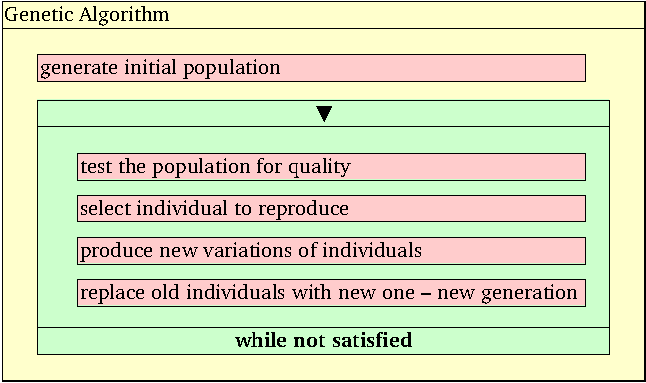
\includegraphics[page=1]{chapter3/GA-kopenogram-crop.pdf}    
%    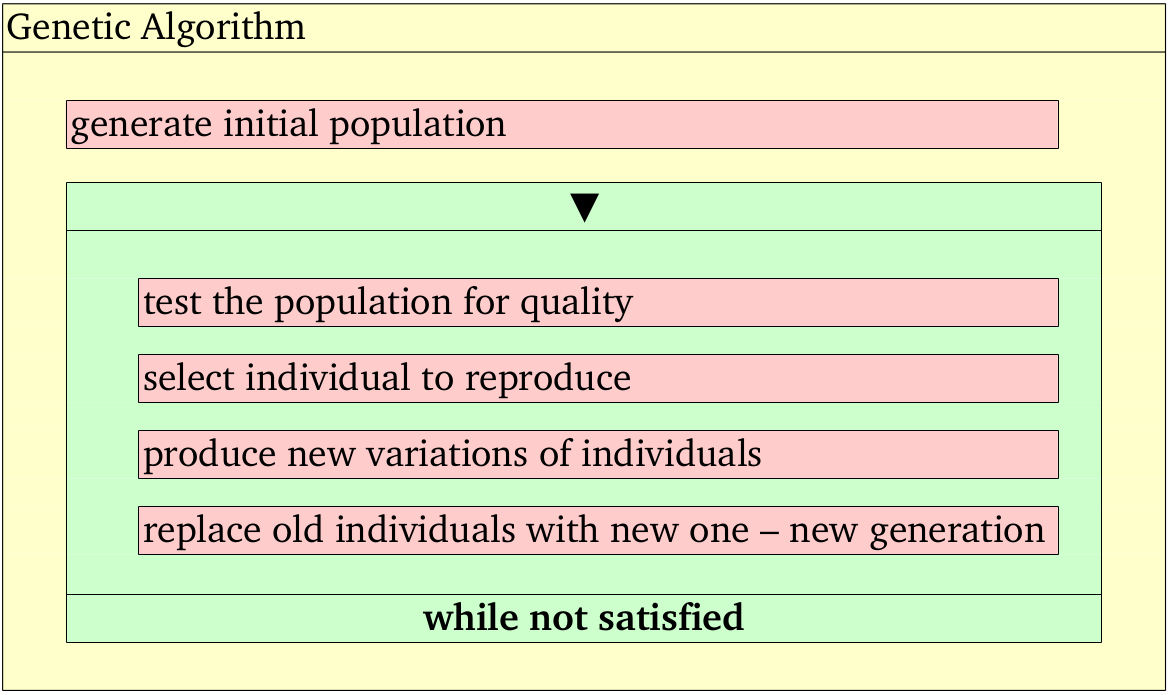
\includegraphics[width=0.5\textwidth]{chapter6/GA-kopenogram.png}
    \caption{Kopenogram of genetic algorithm. 
    }
    \label{fig:GA-kopenogram}
\end{figure}
\begin{figure}[htb]
    \centering
    \includegraphics[page=2]{chapter3/GA-kopenogram-crop.pdf}    
%    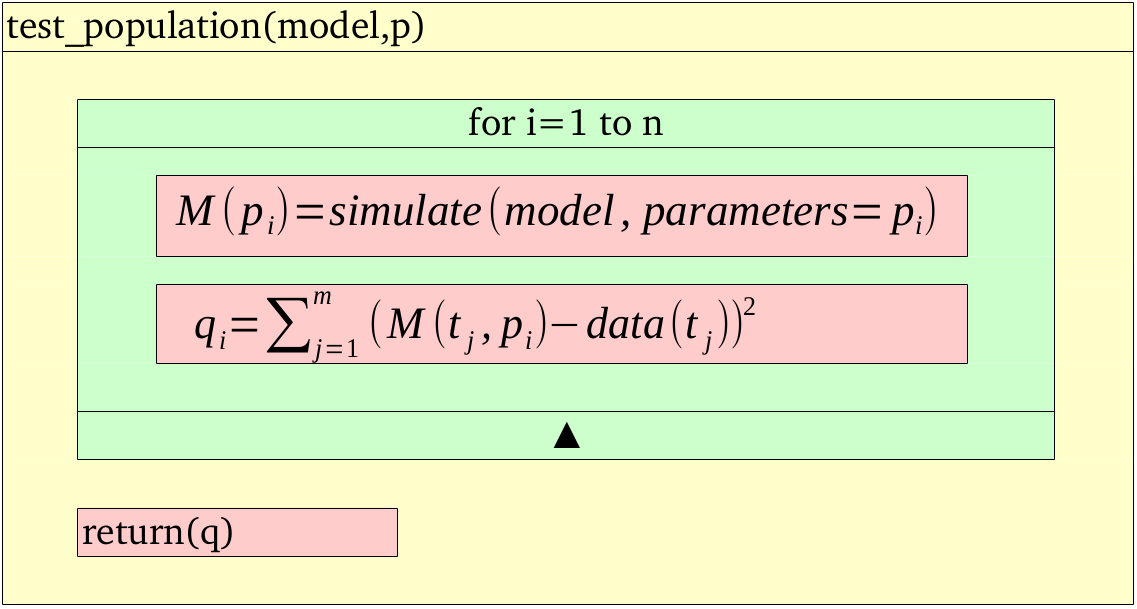
\includegraphics[width=0.5\textwidth]{chapter6/GA-kopenogram2.png}
    \caption{Kopenogram of genetic algorithm and specific test of the population for quality in case of parameter estimation. Model is simulated according to individual $i$ with parameters $p_i$ and the quality $q_i$ is counted per the objective function \ref{eq:parameter}.
    }
    \label{fig:GA-kopenogram2}
\end{figure}
Evolutionary algorithms can be used as heuristic strategy for finding global minimum or maximum and it can be used to estimate the parameters of the model. Genetic algorithm a type of evolutionary algorithm which encodes individuals as binary string was introduced e.g. by Holland\cite{Holland1975} and the algorithm steps are schematically presented in figure \ref{fig:GA-kopenogram}.

The iteration within the loop "$\blacktriangledown \ldots$ \emph{while not satisfied}" depends on previous iteration, thus it cannot be parallelized.
The step \emph{test the population for quality} has algorithmical structure in fig.\ref{fig:GA-kopenogram2} for parameter estimation tasks. Each iteration in the loop "\emph{for i=1 to n}" is independent and a therefore loop parallelism (section \ref{sec:parallelprogramming}) can be utilized and implemented here.

%The Amdahl's law in equation \ref{eq:amdahl} can be used to estimate  the theoretical speedup limitation for the specific model and potential gain for identifying different types of models can be stated. We assume that the simulation of the model with any parameters will take the same time, even this is not generally true as the non-linear models and numerical methods may cause different steps to be performed for different parameter values. 

%The specific fraction $\alpha$ for the model determines the level of scalability of the model within the parallelized system. For the complex models the $\alpha$ will decrease. The specific estimates of the fraction $\alpha$ and it's influence on the scalability and results are presented in section \ref{sec:resultsestimation}.

\subsubsection{Architecture of system for parameter estimation}
\begin{figure}[hbt]
    \centering
     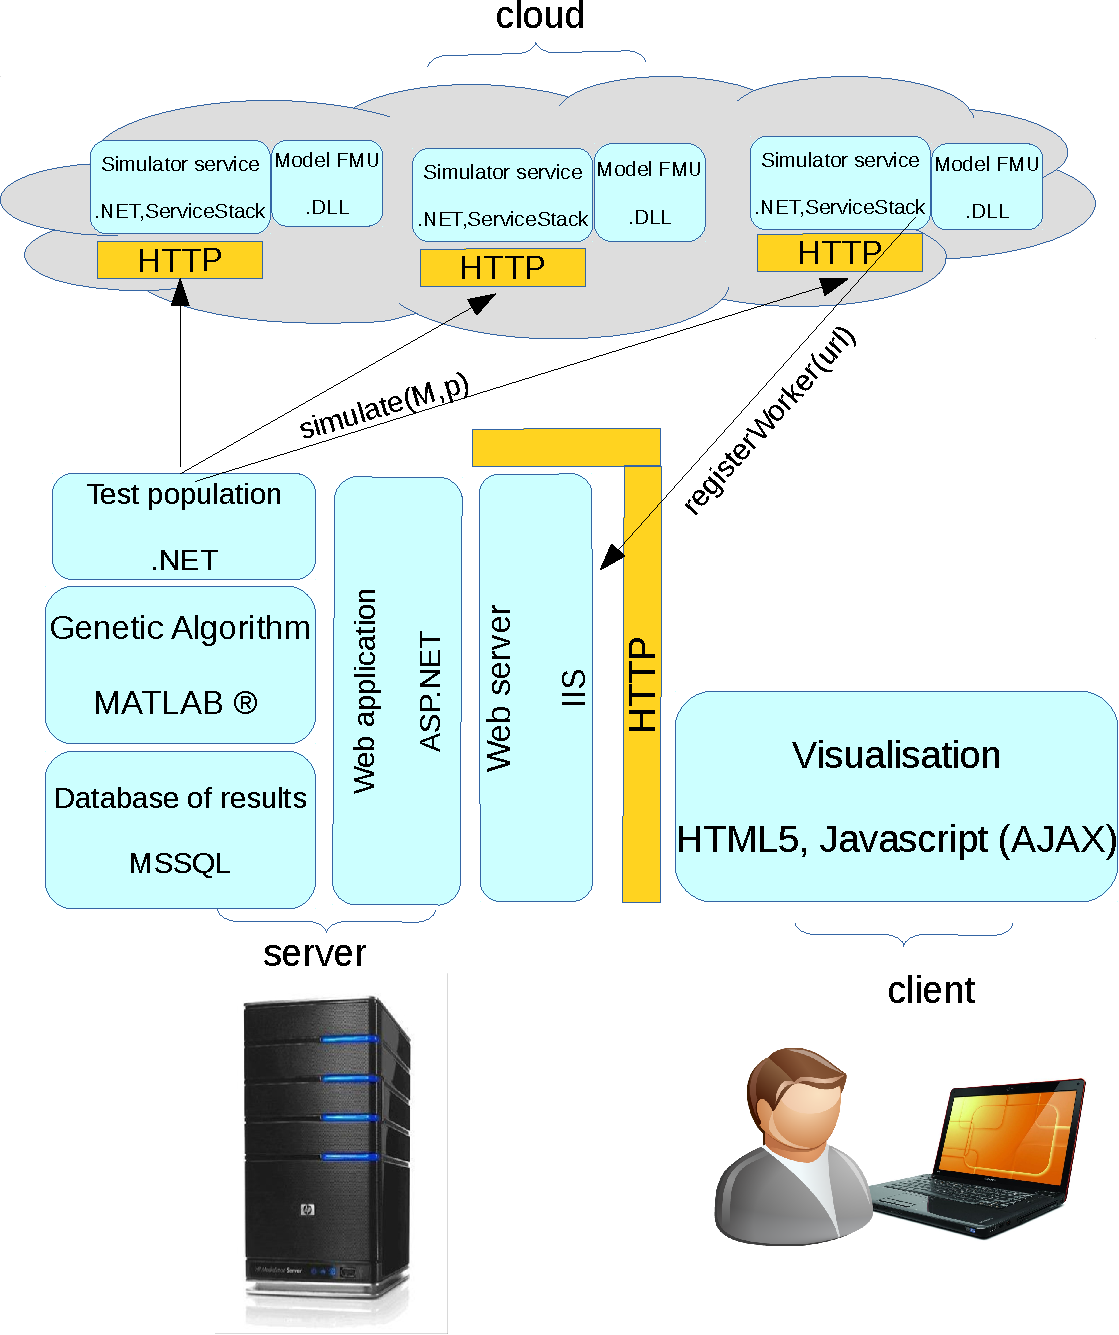
\includegraphics[page=1,width=0.75\textwidth]{chapter3/architekturaestimation-crop.pdf}  
    \caption{Architecture of the system employing genetic algorithm and distributing the \emph{simulate} task into cloud computing environment.}
    \label{fig:architectureestimation}
\end{figure}
Proposed architecture of the system for parameter estimation (fig. \ref{fig:architectureestimation}) was influenced by the need of some interactivity and overall accessibility for users which is fulfilled by the web UI. The key part of the system in opposite side is a model exported into a binary platform dependent library. 
The specific model of a studied system implemented in Modelica is exported into standard Functional Mockup Unit(FMU) with is standardized XML metadata packaged together with  binary library .DLL (or .SO) following standardized API \cite{Blochwitza}\footnote{\url{https://www.fmi-standard.org/} accessed February 2015}. In the time of writing the thesis the most stable Modelica tool export was Dymola\footnote{\url{http://www.dynasim.se} - Dymola tool, accessed March 2015} export to FMU for MS Windows platform. 

The parallelization is implemented using threads in \emph{test\_population} method which within a loop follows fork/join pattern -- the created threads simultaneously asks for simulation results with a parameter set and main process waits until all results are returned to compute full vector of quality evaluation $q$.

Packaged with .NET ServiceStack framework\footnote{\url{https://servicestack.net/} accessed February 2015} it exposes a simulation functionality as a RESTful web service which can be accessed and orchestrated by the \emph{test\_population} algorithm. The implementation of genetic algorithm is reused from MATLAB \texttrademark and with a database of results in a SQL database is integrated with ASP.NET web application presenting a web user interface and functionality to a user.
The result of applying the methods and deploying the designed system in local cluster and cloud computing infrastructure is described in section \ref{sec:resultsestimation}.

\subsection{Parameter Sweep}
\label{sec:sensitivity}
\begin{figure}[hbt]
    \centering
     \includegraphics[page=4]{chapter3/GA-kopenogram-crop.pdf}    
%    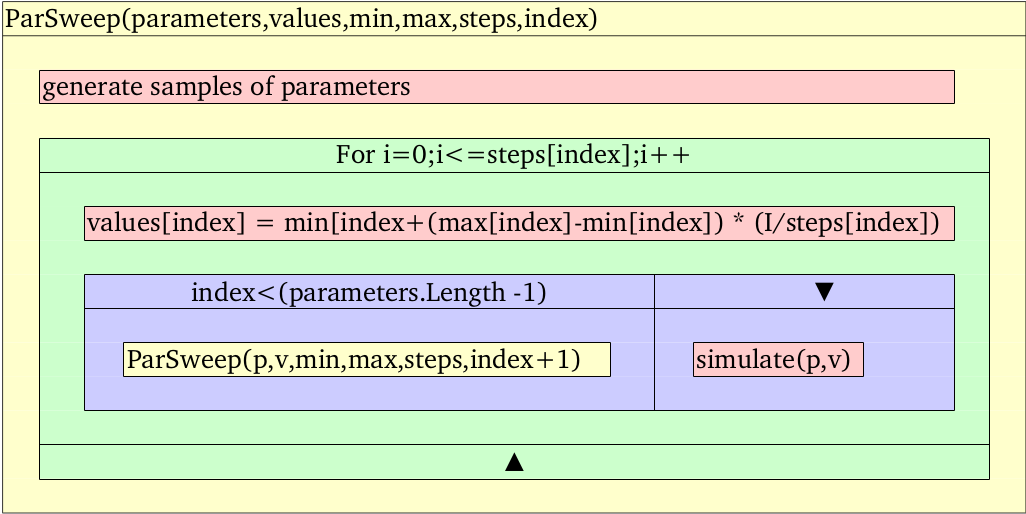
\includegraphics[width=1\textwidth]{chapter3/paramsweepkop.png}
    \caption{Kopenogram of recursive parameter sweep algorithm. $p$,$v$,$min$,$max$ and $steps$ are arrays with the same dimension holding parameter name, value, starting and stoping value and number of steps which needs to be performed between starting and stopping value per each $index$.    
    }
    \label{fig:paramsweep}
\end{figure}

Parameter sweep (PS) is one of the techniques used for sensitivity and uncertainty analysis which is based on changing selected parameters and simulating whole model and quantifying the change on model behavior with different parameters. Uncertainty and sensitivity analysis tries to determine how a change of the value of parameter will contribute to the model output and how the estimation of parameter values are robust to errors of measurement of the real data. Various methods to do uncertainty and sensitivity analysis can be found e.g. in a reviews by Helton et al. \cite{Helton2006} or a books by Saltelli et al.\cite{Saltelli2004,Saltelli2008}. 

Recursive algorithm of parameter sweep for exploring parameter space (in fig.\ref{fig:paramsweep}) generates tremendous number of simulation. Presuming that \emph{simulate} operation takes constant time for any parameters (which is not true in general) the time complexity of PS is $O(\prod_{i=1}^{n}) \text{steps}_i) \approx  O(k^n)$ where $k=\max_{i=1}^n(\text{steps}_i)$ and $n$ is number of parameters to be swept. E.g. for 1000 values for each parameter: $O(1000^n)$. The large number of distinct simulation can take tremendous time on single computer. However, in contrast to parameter estimation, each of the simulation is independent and PS algorithm is determined as embarrassingly parallel and is implemented in many grid-computing projects and workflows e.g. P-Grade portal as published by Kacsuk et al.\cite{Kacsuk2011}.

To perform parameter sweep algorithm on the models of human physiology in Modelica language an export from the Modelica is needed. The FMU standard supported by many tools exports FMU as 

a BOINC platform\cite{Anderson2004}\footnote{\url{http://boinc.berkeley.edu/} accessed February 2015} is customized following the task parallelism and master/worker programming model (reffered in section \ref{sec:parallelprogramming}). The Modelica model exported as FMU for Windows platform is integrated with BOINC wrapper and as a whole it is integrated into BOINC platform deployed on a server as seen in fig. \ref{fig:paramsweeparch}. 

\begin{figure}[htb]
    \centering
     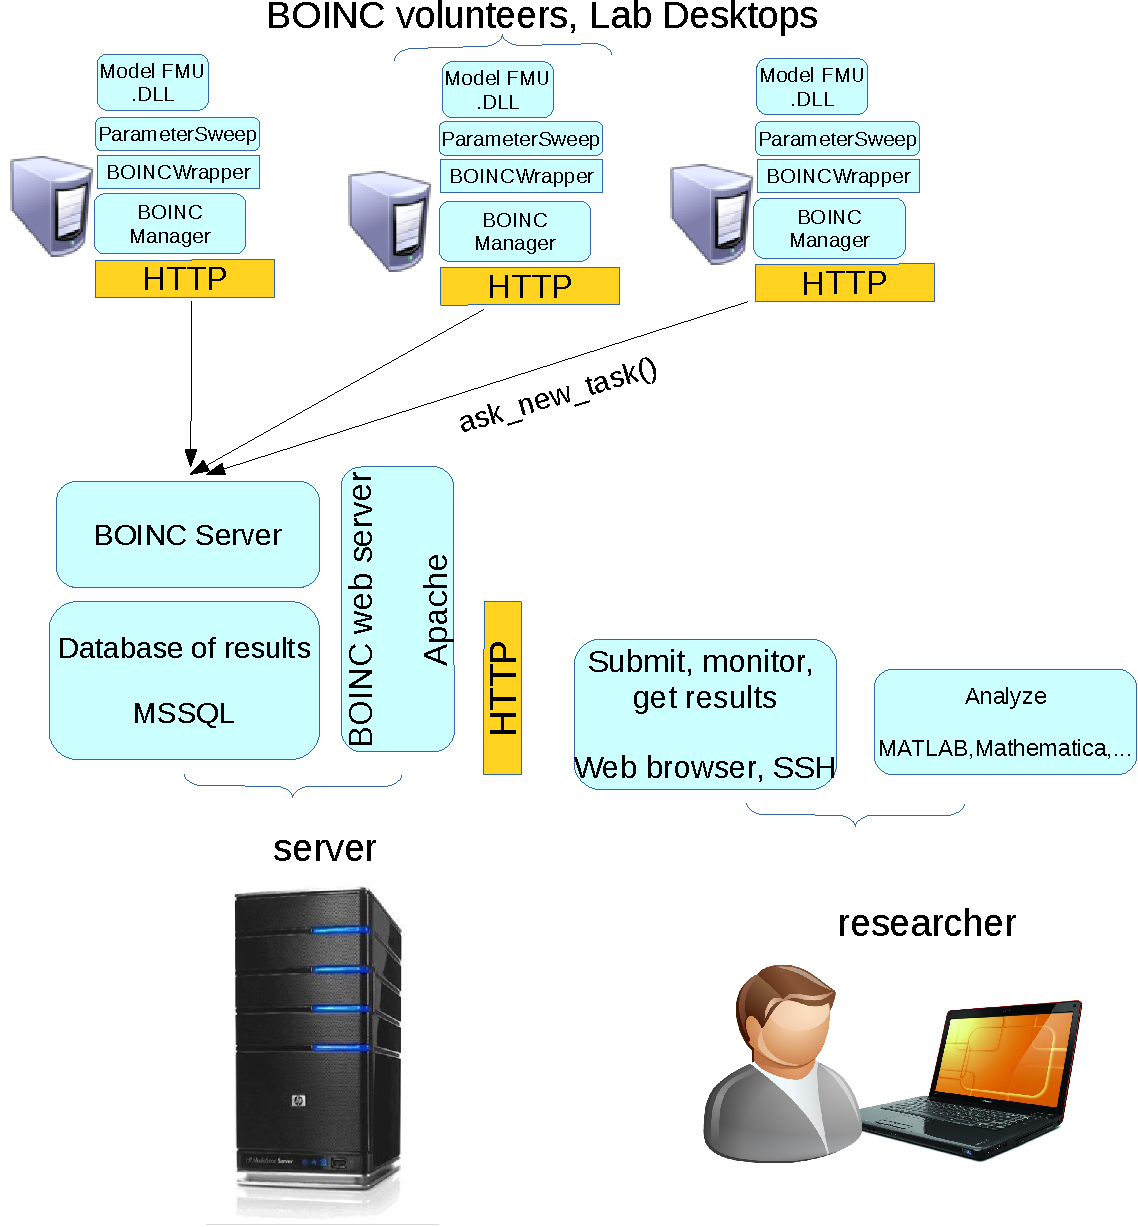
\includegraphics[page=1,width=0.75\textwidth]{chapter3/architekturaparamsweep-crop.pdf}    
%    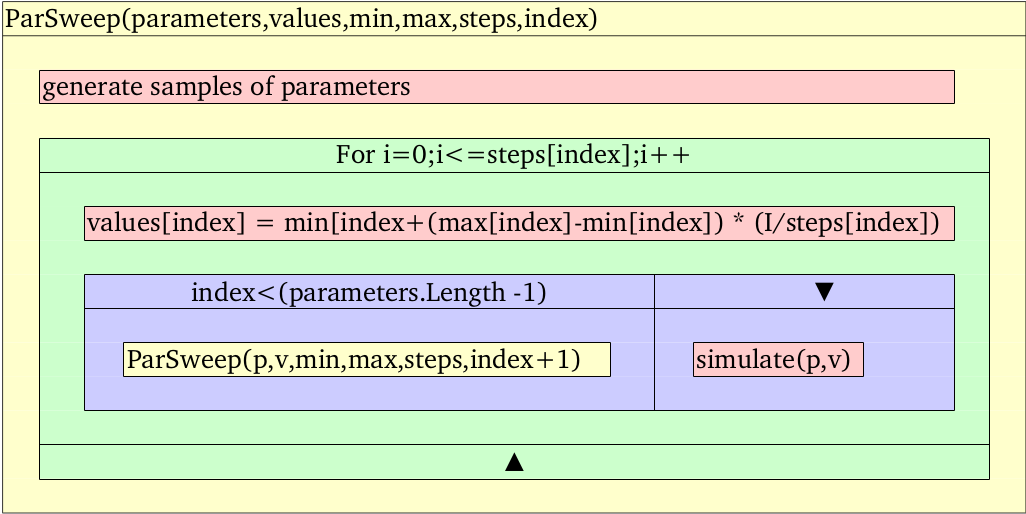
\includegraphics[width=1\textwidth]{chapter3/paramsweepkop.png}
    \caption{Architecture of parameter sweep application. The whole parameter space is divided into smaller spaces which are resolved by the BOINC workers}
    \label{fig:paramsweeparch}
\end{figure}

The results are described in section \ref{sec:resultsestimation}.

%The paper \cite{Kulhanek2011} \emph{From Educational Models Towards Identification of Physiological Systems} in Appendix~\ref{app:fromeducational} describes desktop grid system BOINC and deployment for parameter estimation mentioned in previous chapter. However, per the high latency of BOINC solution, the of the specific Modelica model exported into Windows executable into BOINC client. 
